\documentclass{beamer}

\usepackage{amsmath}
\usepackage{amssymb}
\usepackage{tikz}
\usepackage{pgfplots}
\usepackage{bm}

\title{Least-Square Problem}
\subtitle{The ``Whole"  Point of Chapter 6}
\author{Ahmed Mohammed}
\institute{Georgia Institute of Technology}
\date{PLUS Session, Fall 2023}

\usetheme{Copenhagen}
\usefonttheme{serif}

\renewcommand{\vec}[1]{\bm{#1}}
\DeclareMathOperator{\proj}{proj}
\DeclareMathOperator{\colspace}{Col}


% from https://tex.stackexchange.com/a/75550/227665
\makeatletter
\let\save@measuring@true\measuring@true
\def\measuring@true{%
  \save@measuring@true
  \def\beamer@sortzero##1{\beamer@ifnextcharospec{\beamer@sortzeroread{##1}}{}}%
  \def\beamer@sortzeroread##1<##2>{}%
  \def\beamer@finalnospec{}%
}
\makeatother

\AtBeginSection[]
{
    \begin{frame}
        \frametitle{Table of Contents}
        \tableofcontents[currentsection]
    \end{frame}
} % https://statisticaloddsandends.wordpress.com/2019/02/18/beamer-inserting-section-slides-before-each-section/

\begin{document}
	\begin{frame}
		\maketitle
	\end{frame}

	\section{Open Activity: Review}
	\begin{frame}
		\frametitle{Motivation}
		\begin{enumerate}[<+(1)->]
			\item \(A\vec{x} = \vec{b}\) could be inconsistent.
			\item Try to solve for the \textit{best approximation} of \(\vec{b}\) by the columns of \(A\).
			\item Recall the following theorem:
				\begin{theorem}[Best Approximation Theorem]
					The projection of a vector \(\vec{y}\) into a subspace \(W\) is the closest vector in \(W\) to \(\vec{y}\).
				\end{theorem}
			\item What is \(W\) and \(\vec{y}\) in our case?
		\end{enumerate}
	\end{frame}

	\begin{frame}
		\frametitle{Motivation \textit{Cont.}}
		 \begin{enumerate}[<+(1)->]
			\item So now we solve for \(A\vec{\hat{x}} = \vec{\hat{b}} = \proj_{\colspace{A}}\vec{b}\).
		\end{enumerate}\pause

			\begin{definition}
				Each solution \(\vec{\hat{x}}\) for \(A\vec{\hat{x}} = \vec{\hat{b}}\) is called a least-squares solution.*
			\end{definition}
			Remark: There might be more than one least-squares solution.
	\end{frame}

	\begin{frame}
		\frametitle{Motivation \textit{Cont.}}
		Calculating the projection of a vector onto a subspace is really simple! \pause 
		\begin{align*}
			\proj_{\colspace A} \vec{b} &= \frac{\vec{a}_1 \cdot \vec{b}}{\vec{a}_1 \cdot \vec{a}_1}\vec{a}_1 + \frac{\vec{a}_2 \cdot \vec{b}}{\vec{a}_2 \cdot \vec{a}_2}\vec{a}_2 + \cdots + \frac{\vec{a}_p \cdot \vec{b}}{\vec{a}_p \cdot \vec{a}_p}\vec{a}_p \\[0.5em] \pause
								 &= \underbrace{\begin{bmatrix}\vec{a}_1 & \vec{a}_2 & \dots & \vec{a}_p\end{bmatrix}}_{A}\underbrace{\begin{bmatrix}\frac{\vec{a}_1 \cdot \vec{b}}{\vec{a}_1 \cdot \vec{a}_1} \\[0.5em] \frac{\vec{a}_2 \cdot \vec{b}}{\vec{a}_2 \cdot \vec{a}_2} \\[0.5em] \vdots \\[0.5em] \frac{\vec{a}_p \cdot \vec{b}}{\vec{a}_p \cdot \vec{a}_p}\end{bmatrix}}_{\vec{\hat{x}}} = \vec{\hat{b}} \pause
		\end{align*}

		We've found the vector \(\vec{\hat{x}}\) such that \(A\vec{\hat{x}} = \vec{\hat{b}}\). So, are we done? 
	\end{frame}

	\begin{frame}
		\frametitle{Motivation \textit{Cont.}}
		No! 
		\begin{enumerate}
			\item<2-> Works for \emph{orthogonal basis} only, not \emph{any} basis.
			\item<3-> We have no guarantee that the columns of \(A\) are linearly independent, let alone orthogonal.
		\end{enumerate}
	\end{frame}

	\begin{frame}
		\frametitle{The Work Around: The Normal Equations}
		They are:
			\[A^TA\vec{x} = A^T\vec{b}.\]\pause

		Turns out that each vector \(\vec{x}\) satisfying the above equation also satisfies the equation 
		\(A\vec{x} = \proj_{\colspace A} \vec{b}\).

		Therefore, a solution to the norm equations \emph{also} counts as a least-square solution.
	\end{frame}
	
	\section{Application}
	\begin{frame}
		\frametitle{Use}
		Least-square problems come up in simple \emph{linear regression} problems. \pause

		\begin{enumerate}
			\item<2-> We have data points \((x_1, y_1), (x_2, y_2), \dots, (x_n, y_n)\) that we wish to connect with curve.
			\item<3-> We chose a linear model. For example, \(y_i = \beta_0 + \beta_1 x_i\) or \(y_i = \beta_0 + \beta_1 x_i^2\) or
					\(y_i = \beta_0 + \beta_1x_i + \beta_2 x_i^2\).
			\item<4-> We try to find what values for \(\beta_0\), \(\beta_1\), \(\dots\), \(\beta_j\) will yield the graph with the least amount of ``error".
		\end{enumerate}
	\end{frame}
	
	\begin{frame}
		\frametitle{Example}
		Find the values for \(\beta_0, \beta_1\) that'll best fit the curve \[y = \beta_0 + \beta_1 x\] to the data points \((1, 2), (2, 3), (3, 3), (5, 5)\). \pause

		\begin{figure}[!h]
			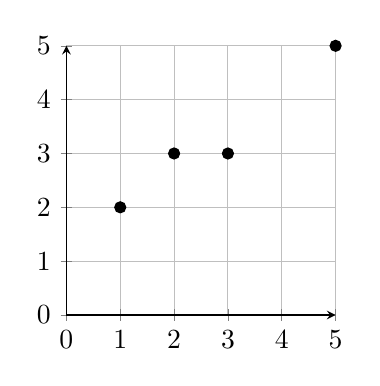
\begin{tikzpicture}
				\begin{axis}[axis lines = left, grid=major, height=5cm, width = 5cm, xmin=0, xmax=5, ymin=0, ymax=5, xtick distance = 1, ytick distance = 1]
					\plot[mark=*, only marks, black] coordinates {(1, 2) (2, 3) (3, 3) (5, 5)};
				\end{axis}
			\end{tikzpicture}
		\end{figure}
	\end{frame}

	\begin{frame}
		\frametitle{Example \textit{Cont.}}
		Find the values for \(\beta_0, \beta_1\) that'll best fit the curve \[y = \beta_0 + \beta_1 x\] to the data points \((1, 2), (2, 3), (3, 3), (5, 5)\).
		\begin{figure}[!h]
			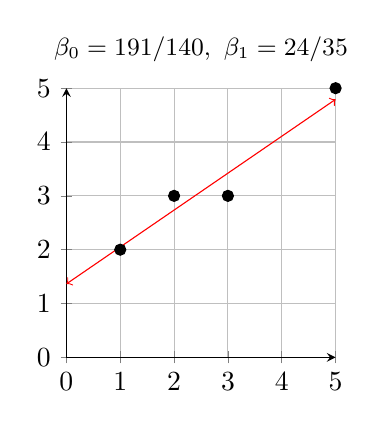
\begin{tikzpicture}
				\begin{axis}[axis lines = left, grid=major, height=5cm, width = 5cm, xmin=0, xmax=5, ymin=0, ymax=5, xtick distance = 1, ytick distance = 1, title={\small \(\beta_0 = 191/140, \ \beta_1 = 24/35\)}]
					\plot[mark=*, only marks, black] coordinates {(1, 2) (2, 3) (3, 3) (5, 5)};
					\addplot[<->, red, domain=0:5] {191/140 + 24/35 * x};
				\end{axis}
			\end{tikzpicture}
		\end{figure}
	\end{frame}

	\begin{frame}
		\frametitle{Model Choice}
		Note that a different model could've been chosen for the previous problem, and as long as the model is linear in the parameters, nothing of the steps would change.
	\end{frame}

	\begin{frame}
		\frametitle{Simpler Question}
		Find the least-square solution for the system \[\begin{bmatrix}1 & 1 \\ 0 & 0 \\ -1 & 1 \\ 0 & 0\end{bmatrix}\vec{x} = \begin{bmatrix}1 \\ 2 \\ 4 \\ 1\end{bmatrix}.\]
	\end{frame}

	\begin{frame}
		\frametitle{A ``Harder" Example}
		Find the value(s) for the parameters \(\alpha, \beta\) that'll best fit the curve.
		\[y = \alpha x^2 + \beta\] to the data points \((-1, 1), (1, 3), (1, 2), (1, 1)\).
	\end{frame}
\end{document}
